\chapter{Les perspectives du projet}
Le projet est toujours en cours de développement, et la production des données continue jusqu’en 2025. Cela invite à s’interroger sur l’avenir du projet, à la fois pour les données produites, mais aussi pour la technologie qui a été élaborée pour. Sur le plan des données, le projet se concentre sur l'amélioration de l'appariement, c'est-à-dire la capacité à relier entre elles diverses informations pour permettre, des analyses approfondies des trajectoires individuelles. Concernant la technologie, notamment les avancées réalisées en HTR, on peut envisager qu'elles puissent être appliquées à d'autres corpus, ouvrant ainsi de nouvelles perspectives pour l'exploitation de données historiques ou manuscrites.

    \section{Le chantier de l'appariement}

L’appariement, ou "linking" est la dernière phase du projet. A partir des données numérisées et entrées dans la base de données, l’objectif est de pouvoir retracer la trajectoire d’un individu, sur plusieurs décennies. On l’a déjà mentionné, Lionel Kesztenbaum a porté un projet similaire avec Jérôme Bourdieu, l’enquête TRA. Le travail effectué utilise les méthodes traditionnelles de la démographie historique, en se basant sur les informations d’état civil, les registres fiscaux et les tables décennales et vise un échantillon de la population : les Français portant un patronyme commençant par TRA. En considérant que cet échantillon est représentatif de la population française, les résultats visent à comprendre la répartition des richesses sur le territoire. Pour enrichir les données, l'enquête a utilisé l'appariement, c'est-à-dire la correspondance entre différentes sources pour un même individu à différentes étapes de sa vie. Cela permet de reconstituer les trajectoires de vie complètes des individus.  
Cette enquête s’inscrit à la suite de la fameuse enquête "3000 familles" lancée par Jacques Dupâquier en 1980. L’idée était ici aussi de retrouver des trajectoires géographiques et sociales d’individus français au XIXe siècle. Comme on l’a déjà dit, l’histoire démographique était composée essentiellement de monographie sur un territoire en particulier, en se basant sur les registres paroissiaux. Avec l’enquête des 3000 familles, on explore davantage de territoires, avec des données déjà collectées par les familles interrogées, qui avaient réalisé la généalogie de leur famille. Malgré son ambition, l'enquête a été confrontée à des défis, notamment en termes de reconstitution complète des généalogies. La complexité des sources, les destructions d'archives, et les difficultés à suivre tous les individus dans le temps ont limité son l'ampleur. SocFace va au-delà de ces difficultés, en mettant en œuvre des moyens beaucoup plus conséquents, afin d’étendre la collecte des données sur l’ensemble du territoire et non plus sur quelques familles ou individus qui serviraient d’échantillon, mais bien sur l'ensemble des Français.\\
L’objectif est donc de construire un deuxième étage de la base de données, et de travailler sur des algorithmes permettant d’identifier un individu à travers le temps. C’est un immense défi, qui va rencontrer de nombreuses difficultés : identifier un individu, à travers les homonymes, s’assurer de le retrouver sur plusieurs recensements, limiter le nombre d’erreurs. Cette base de données n’est pas encore construite et les processus sont encore à l’étude. A ce jour, il a été décidé d’utiliser le module \textit{H Link}, sous Python, qui permet d’utiliser et de manipuler des hyperliens. C’est un outil largement utilisé pour le webscrapping mais aussi pour IPUMS, le projet similaire à SocFace porté par l’université du Minnesota. 
Permettre de retrouver la trajectoire d’un individu à l’échelle d’une vie et d’un territoire national est une grande avancée pour la démographie historique. L’exhaustivité des informations données – même si elle n’est pas de 100\% - donne une image beaucoup plus précise de la population française sur 100 ans, permettant d’améliorer les études sociales et démographiques des historiens.\\

L’appariement est une exploitation des données. Mais il est intéressant de réfléchir à l’exploitation de la technologie elle-même. 

    \section{Une technologie appliquée à d'autres coprus?}

Au-delà de l’appariement, les données brutes vont aider les chercheurs à affiner leurs analyses sur des périodes plus longues et sur une plus grande surface géographique. Bien que les informations recueillies tous les cinq ans soient assez limitées, la stabilité des enquêtes sur près de cent ans permet d’opérer des comparaisons sur une longue période. Par ailleurs, on peut être un peu plus assuré de l’exhaustivité des résultats qu’avec un travail manuel effectué par un chercheur ou par des passionnés qui indexeraient à la main les listes de recensement d’un espace ou d’une zone déterminée. Le processus mis en place n’exclue pas les erreurs, mais elles sont limitées. On peut supposer que ces informations pourront être par la suite croisée avec d’autres données : les registres militaires, les registres fiscaux. Cela pourra améliorer encore plus la connaissance de notre histoire.
Par ailleurs, SocFace permet d’améliorer considérablement les résultats de l’HTR. On a vu que désormais, on pouvait traiter un nombre d’images de grande ampleur, et en retirer des millions de données. Il serait intéressant d’appliquer cette méthodologie à l’OCR et d’appliquer cette technologie à d’autres types de sources. On sait que SocFace est rendu possible car les modèles de recensement sont sensiblement identiques d’un dénombrement à l’autre. Ainsi, les entraînements des modèles sont assez proches pour l’ensemble du corpus. On peut donc penser à des sources qui respectent également un même type d’agencement du texte d’une année à l’autre. Par exemple, Les \textit{Comptes Généraux de la justice criminelle}, publiés en France de 1825 à 1978. Ces énormes livres, publiés en deux volumes chaque année, reprennent les comptes rendus des différentes cours de justice afin d’élaborer un tableau de bord permettant un suivi précis des tribunaux. Le nombre de données est donc considérable, et serait une mine d’information pour les historiens de la période. 
Voici un exemple, qui montre bien que le nombre de données contenues en une page est important : 

\begin{figure}[H]
    \centering
    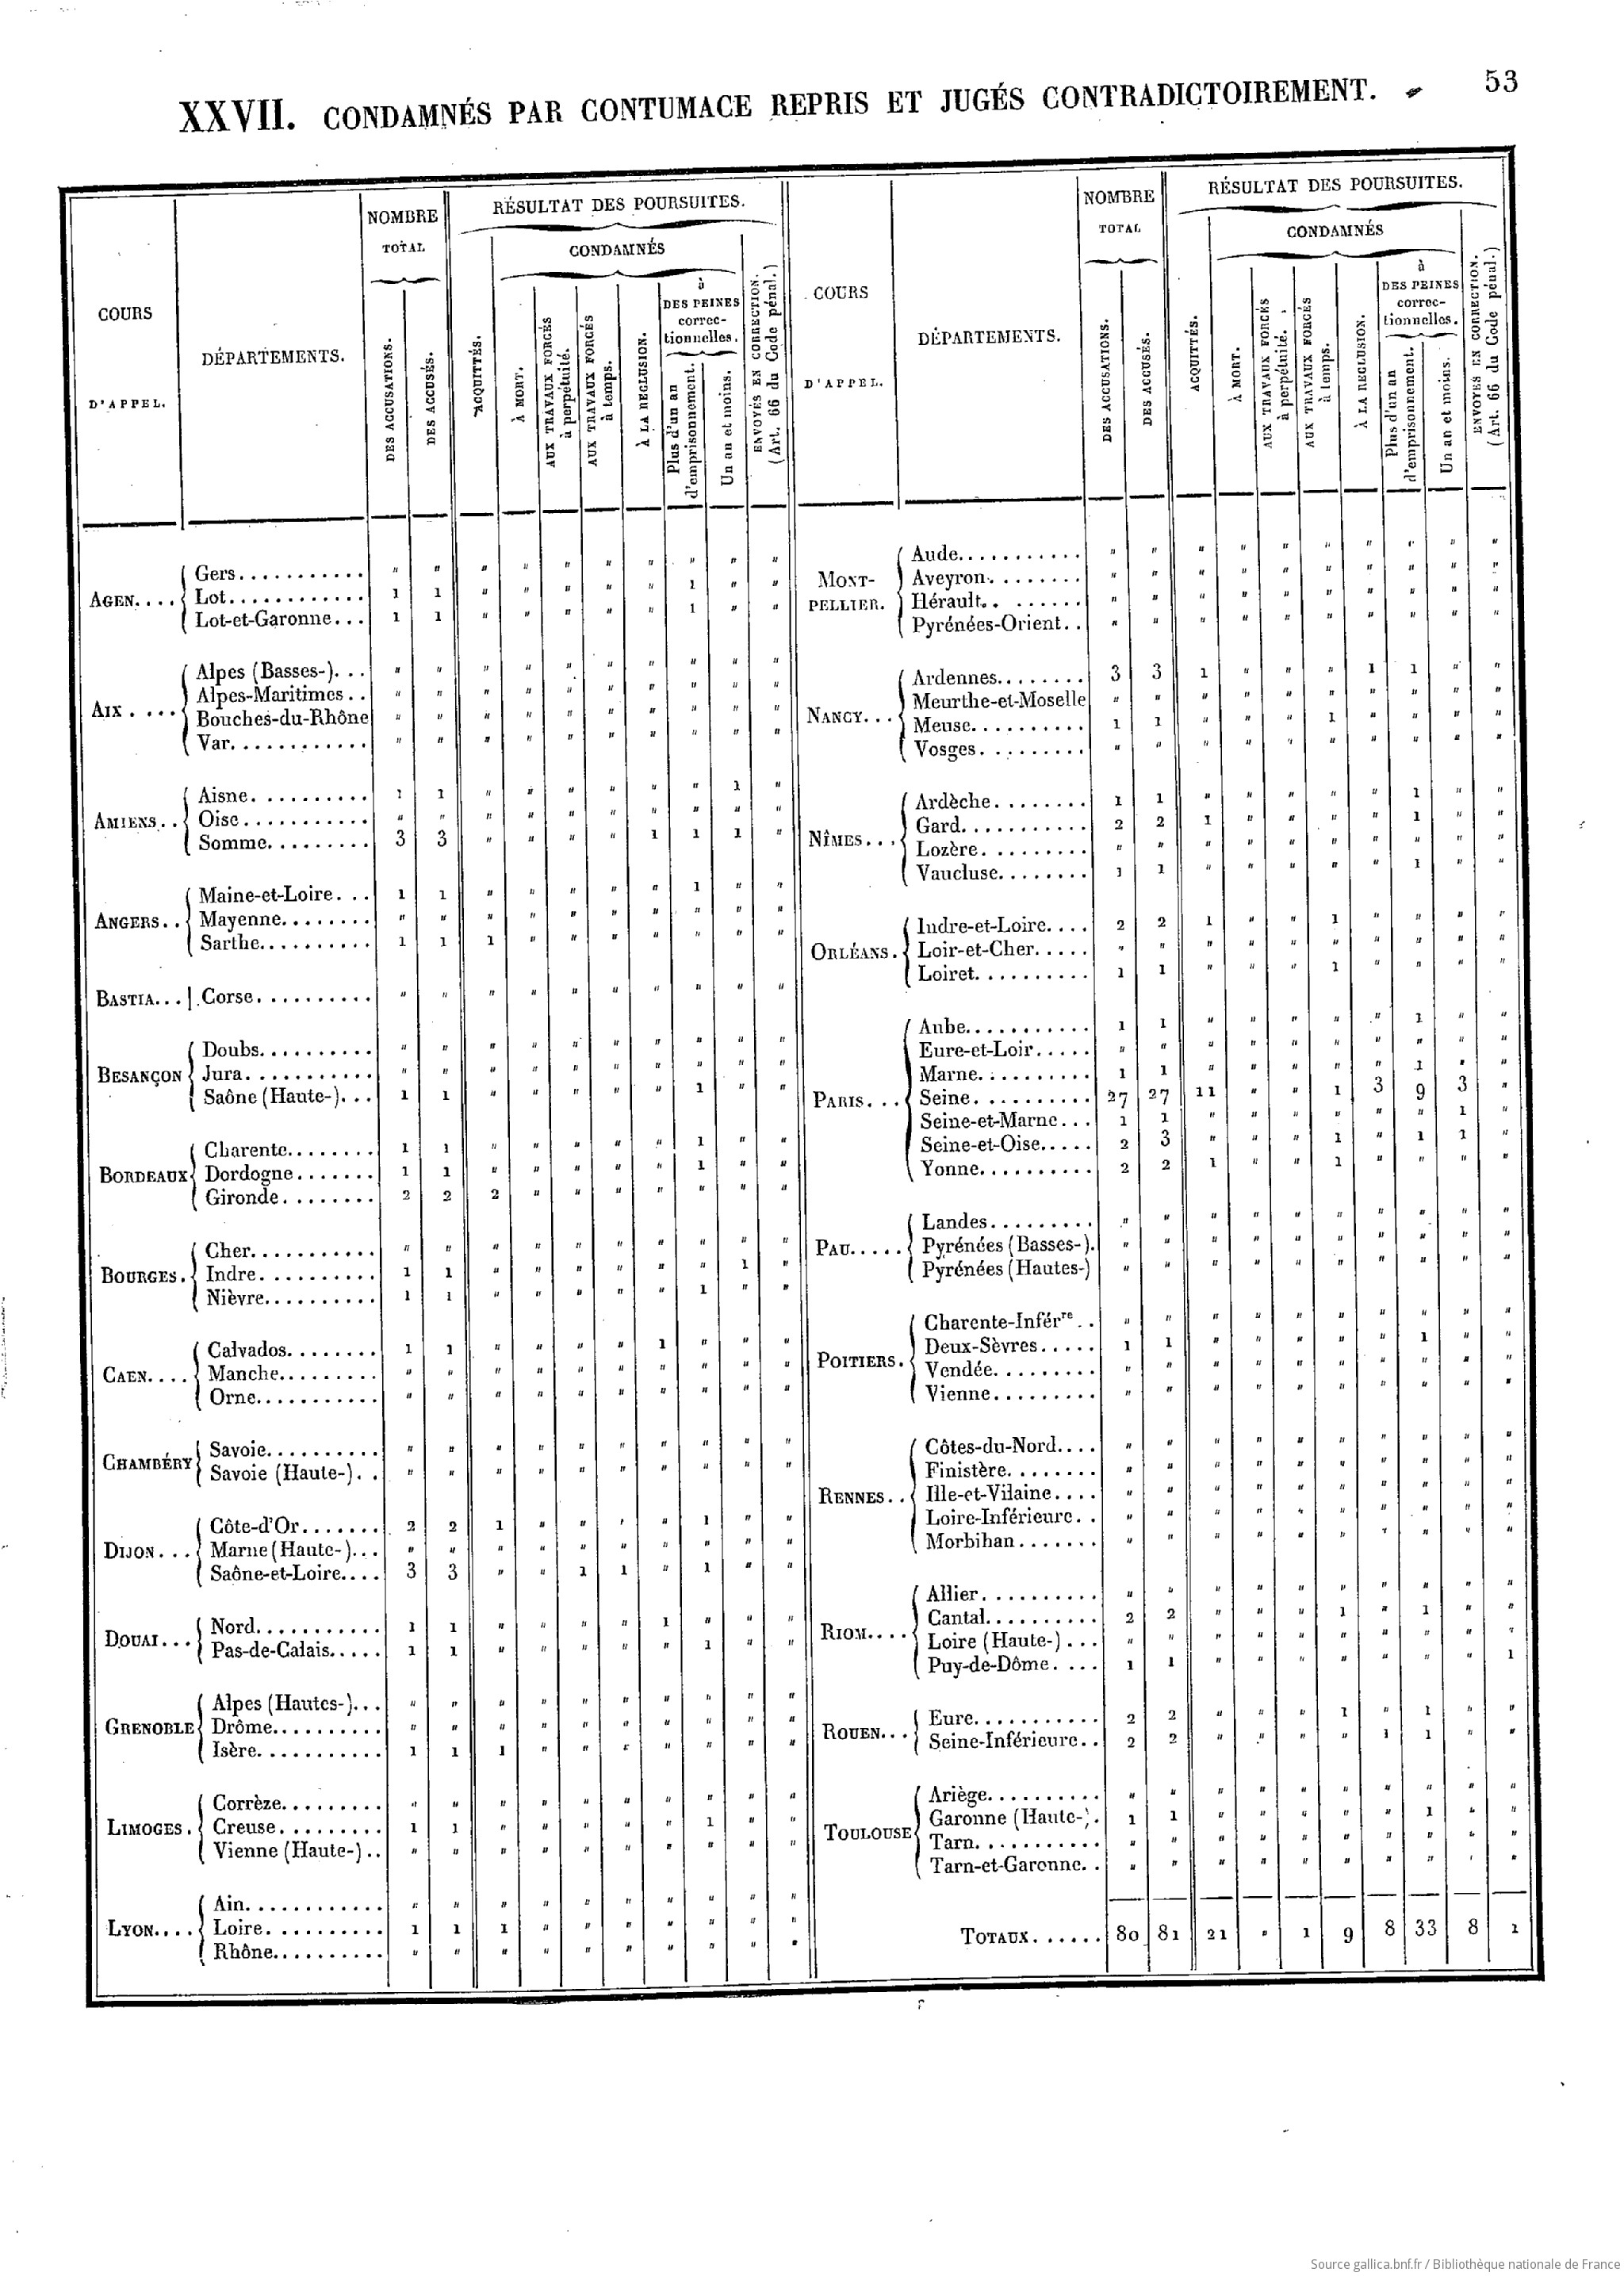
\includegraphics[width=0.7\linewidth]{Figures/Partie 3/Fig.3.3 - Compte Général.jpeg}
    \caption{Extrait du Compte Général pour 1887}
    \textit{Crédit : Gallica}
    \label{fig:Fig.3.3}
\end{figure}

\clearpage
En 1887, on compte 131 pages pour le \textit{Compte}, mais certaines années vont jusqu’à 300 pages. On voit aussi qu’il peut y avoir une difficulté sur la délimitation des zones, sujet qui a été creusé par les équipes de SocFace. 
Un projet de recherche a été mené en 2010, portant d’une part sur la saisie manuelle d’un ensemble de série extraite de ces livres, et d’autre part sur l’analyse des données ainsi obtenues\footnote{\fullcite{Sgard}}. Selon le chercheur en charge du projet, Jérôme Sgard, ces comptes ont été très peu exploités : 
\begin{quote}
    \textit{"Produit typique de l’Etat français à la fois centralisé, bureaucratique et technocratique, les Comptes de l’Administration de la Justice publiés annuellement à partir des années 1830 sont une des sources quantitatives les plus anciennes et des plus fiables disponibles sur l’histoire du pays. Or non seulement elles sont peu utilisées, en outre elles n’ont à peu près jamais été saisies de manière systématiques. Seuls quelques chapitres précis en matière criminelle, ou bien en matière de divorce ou de suicides ont fait l’objet de reconstitutions en séries temporelles de longue durée."}
\end{quote}

Il mentionne des études ponctuelles, par Emile Durkheim dans son étude sur \textit{Le suicide} en 1893 ou encore Michel Foucault pour \textit{Surveiller et Punir} en 1973. Ce genre de sources sérielles serait donc très intéressants à exploiter, particulièrement pour les informations qu’elles peuvent fournir pour les chercheurs et démographes. Ce projet a été financé par l'institut CDC pour la recherche\footnote{\href{Institut CDC pour la recherche}{https://fonda.asso.fr/institut-cdc-pour-la-recherche}}, mais les données issues du projet ne sont pas accessibles au grand public. 
Cet exemple serait une adaptation à des outils d’océrisation, mais concernant la technologie HTR, on peut penser que l’on pourrait appliquer cette technologie à d’autres corpus. La difficulté est la qualité du scripteur. Il faudrait donc un corpus appartenant à un même scripteur, avec des données d’entraînement de qualités, sur une grande variété de mots. On pourrait penser au manuscrit d’un auteur ou bien aux lettres d’un seul et même individu.\\

Le chantier d'appariement mis en œuvre par SocFace marque une nouvelle étape dans l'exploitation des données historiques, permettant une reconstitution fine des trajectoires individuelles. Au-delà de son application à la démographie historique, cette technologie ouvre des perspectives prometteuses pour d'autres corpus de données, tels que les archives judiciaires ou les manuscrits d'auteurs. En intégrant des outils d'OCR et d'HTR, SocFace non seulement enrichit la compréhension de notre passé, mais offre également un modèle adaptable pour d'autres domaines de recherche, renforçant ainsi les capacités des sciences sociales à analyser des données massives et variées.
